\documentclass{article}
\usepackage[margin=2.5cm, top=4cm, headheight=25pt]{geometry}
\usepackage{amsmath, amssymb, enumitem, fancyhdr, graphicx}
\usepackage[indent=20pt]{parskip}
\usepackage[hidelinks]{hyperref}
\usepackage{xcolor}
\usepackage{listings}
\usepackage{subcaption}
\usepackage{url}
\usepackage[most]{tcolorbox}
\usepackage{lastpage}

\tcbuselibrary{listingsutf8} % Support for lstlistings within tcolorbox

\newtcolorbox[auto counter, number within=section]{question}[1][]{%
    colframe=gray!80,                      % Dark gray frame
    colback=gray!5,                       % Light gray background
    coltitle=black,                        % Black title
    title=\textbf{Question~\thetcbcounter}, % Bold title
    fonttitle=\bfseries\large,             % Subtle title font size
    rounded corners,                   % Slightly more rounded corners
    boxrule=0.25mm,                         % Thinner border for a sleek look
    enhanced,                              % Enhanced box features
    attach boxed title to top left={xshift=2mm, yshift=-2mm},
    boxed title style={colframe=gray!80, colback=gray!5, boxrule=0.25mm},
    % Title styling
    #1
}

\bibliographystyle{IEEEtran}
\graphicspath{{./images/}}

% -- Custom Variables --
\def\me{Rajdeep Gill 7934493}
\def\course{ECE 3760}
\def\labsection{A01}
\def\labno{1}
\def\title{Log Book}

% -- Styling for code snippets --
\lstset{
    basicstyle=\ttfamily\small,           % Basic font style
    keywordstyle=\color{blue},            % Keywords color
    commentstyle=\color{gray},            % Comments color
    stringstyle=\color{teal},             % Strings color
    numbers=left,                         % Line numbers on the left
    numberstyle=\tiny\color{gray},        % Line number style
    stepnumber=1,                         % Line number step
    numbersep=10pt,                       % Space between line numbers and code
    backgroundcolor=\color{lightgray!10}, % Background color
    frame=single,                         % Adds a frame around the code
    breaklines=true,                      % Line breaking for long lines
    captionpos=b,                         % Caption position
    showspaces=false,                     % Don't show spaces
    showstringspaces=false                % Don't show spaces in strings
}
\renewcommand{\lstlistingname}{Code Snippet}

\renewcommand{\arraystretch}{1.2} % For less-ugly tables
\setlength\parindent{0pt}

%----- Samples 
% Questions:
%   \begin{question}[title=Custom Question Title]
%       Question details
%   \end{question}

% Tables:
%   \begin{table}[htbp]
%       \centering
%       \caption{Table Caption}
%       \begin{tabular}{ll}
%           \toprule
%           \textbf{Column 1} & \textbf{Column 2} \\
%           \midrule
%           Row 1 & Row 2 \\
%           Row 3 & Row 4 \\
%           \bottomrule
%       \end{tabular}
%   \end{table} 

% Figures:
%   Single figure:
%       \begin{figure}[htbp]
%           \centering
%           \includegraphics[width=0.5\textwidth]{example-image}
%           \caption{Figure Caption}
%       \end{figure}
%   Multiple figures:
%       \begin{figure}[htbp]
%           \centering
%           \begin{subfigure}[b]{0.5\textwidth}
%               \includegraphics[width=\textwidth]{example-image-a}
%               \caption{First subfigure}
%           \end{subfigure}
%           \begin{subfigure}[b]{0.5\textwidth}
%               \includegraphics[width=\textwidth]{example-image-b}
%               \caption{Second subfigure}
%           \end{subfigure}
%           \caption{Main figure}
%       \end{figure}

\newcommand{\logbookentry}[2]{
    \subsection*{#1 \hfill \textit{#2}} 
}

\begin{document}

% --------------------------------------------------------------------------------
% TITLE
% --------------------------------------------------------------------------------

\begin{center}
    \huge \title

    \vspace{2mm}
    \hrule

    \vspace{4mm}
    \large \me

    \vspace{2mm}
    \large \course~\labsection

    \vspace{2mm}
    \today
\end{center}

\vspace{4mm}
\tableofcontents

% --------------------------------------------------------------------------------
% END TITLE
% --------------------------------------------------------------------------------
\vspace{1cm}
\newpage

\pagestyle{fancy}
\fancyhead[L]{\large Logbook}
\fancyhead[R]{\large \me}

\fancyfoot[C]{Page \thepage~of~\pageref{LastPage}}


% --------------------------------------------------------------------------------
% BODY
% --------------------------------------------------------------------------------
\section{LOGBOOK \#1 START}

\logbookentry{Lab 1 Entry}{January 20, 2025}
Received the board, soldered pins to the board and ensured that the board was working and no short circuits were present.

Installed platformio on VSCode and ensured the extension was working correctly by running a simple serial print program on the board.

The program was first built and then uploaded to the board, and got a successful message in the console as seen in \autoref{fig:success_upload}.

\begin{figure}[ht!]
    \centering
    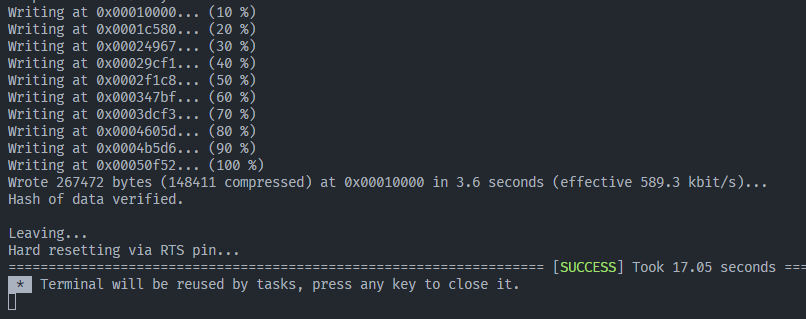
\includegraphics[width=0.8\textwidth]{success_upload.png}
    \caption{Successful upload message in console}
    \label{fig:success_upload}
\end{figure}

\logbookentry{Design Ideas}{January 20, 2025}
During the lab, discussed some ideas for the project. Talked about the basic requirements, what potential ways we can meet the requirements. Need to do more research on how curling actually works to get a better idea of what someone would need to comminicate with their team members to ensure a successful game.

Currently thinking of the skip having a device that can communicate with the two sweepers, having a speed up and slow down button for the sweepers to adjust their speed. The skip would also have a button to indicate when to stop sweeping. On the sweepers side, they would have an LED or a speedometer esque led display to show them how fast they should be sweeping. Since different players might need to sweep at different rates, need to differentiate somehow between the two sweepers. Maybe have two of the same device, but with different colored LEDs or something to indicate which sweeper the skip is talking to. For example, a left and right sweeper device, that connects to the respective sweeper. 

\logbookentry{Individual Design Brainstorming}{January 26, 2025}
A rough sketch of the design I had come up with is provided below. Essentially two sets of controles will be present on the skip's device, one for each sweeper. Along with a display made of LED lights, or other visual indicators to reflect what the sweepers are seeing on there device. 3 buttons will be present, speed up, slow down and an immediate stop button. On the sweeper's device, a line of LED lights or other visual indicators to show a level for the sweeper to sweep at. The skip will be able to adjust the level of the sweeper, and the sweeper will be able to see the level they should be sweeping at.

\begin{figure}[ht!]
    \centering
    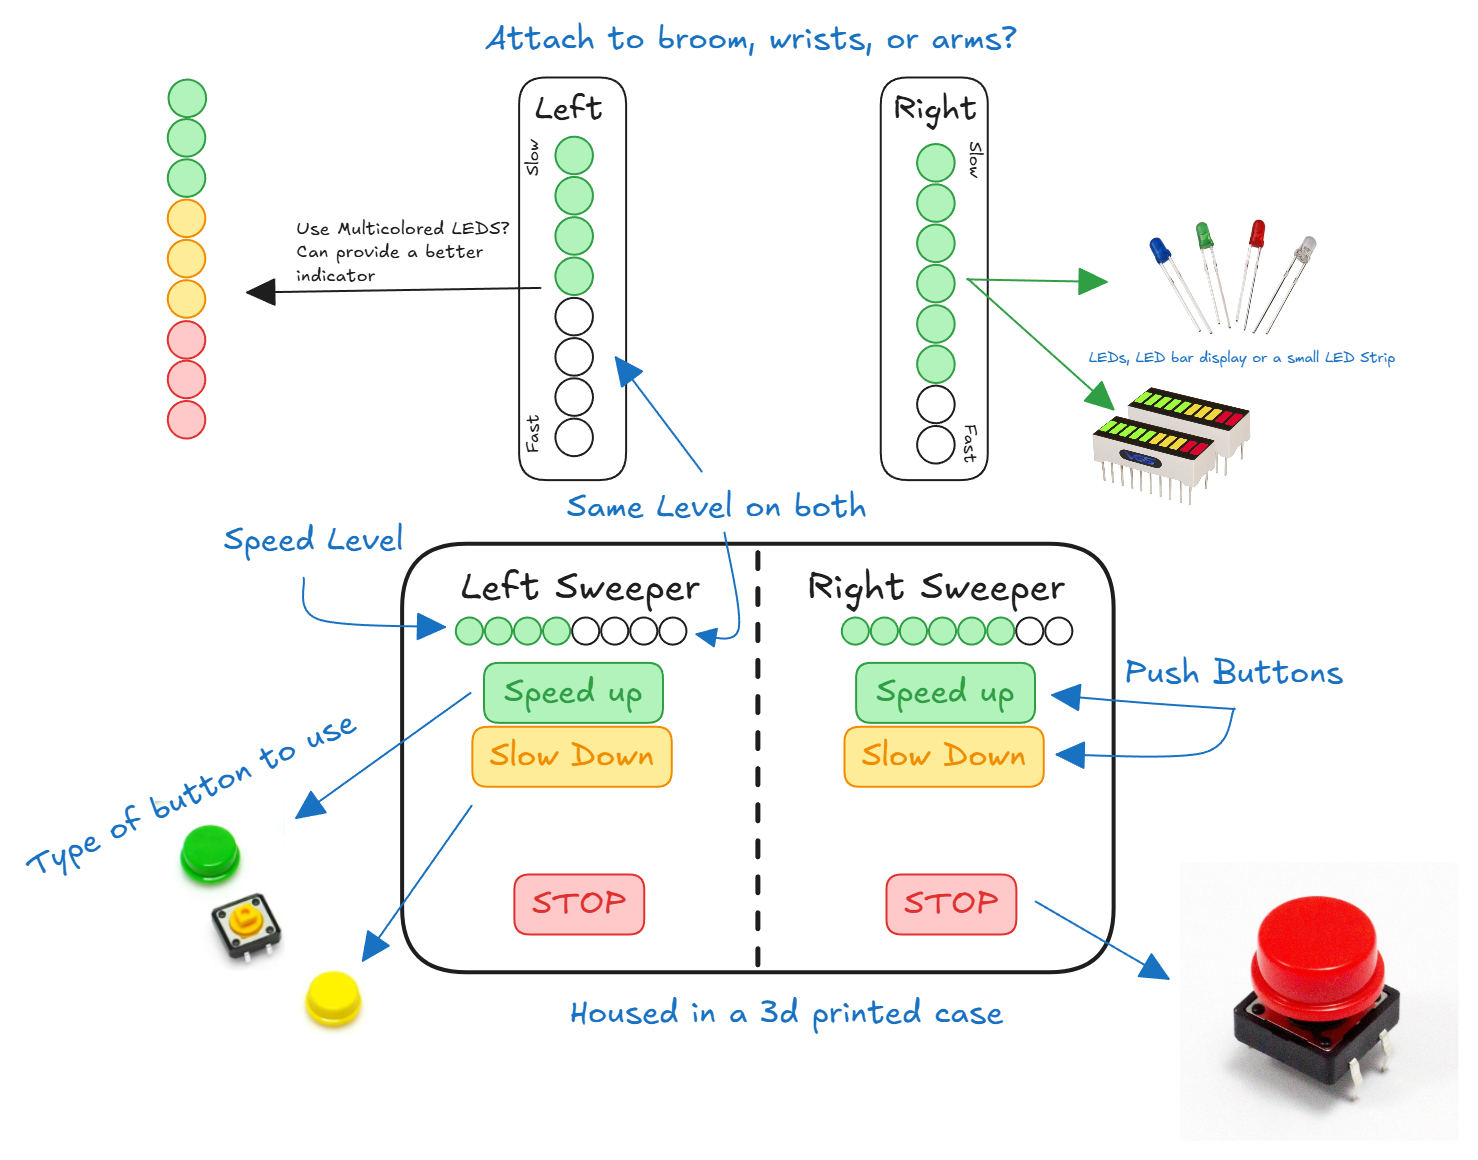
\includegraphics[width=0.7\textwidth]{design_idea1.png}
    \caption{Rough sketch of the design}
\end{figure}
\newpage
The communication between the devices can be done via WiFi as it would have sufficient range to cover the play area. A packet/message structure will need to be defined to ensure the messages are read correctly and by the proper device. A simple message structure could be as follows:

\begin{verbatim}
    <sweeper_id, message_data>
\end{verbatim}
Where \texttt{sweeper\_id} can be a 1 bit for which sweeper, if more than 2 sweepers are present, then we could use 2, 3, 4 bits to represent the sweeper. The message data for each message can be as simple as the level of speed to set the sweeper to, and the sweeper would reply back with an ACK message of the current level they are at to ensure proper synchronization. A simple message-communication diagram is shown below.

\begin{figure}[ht!]
    \centering
    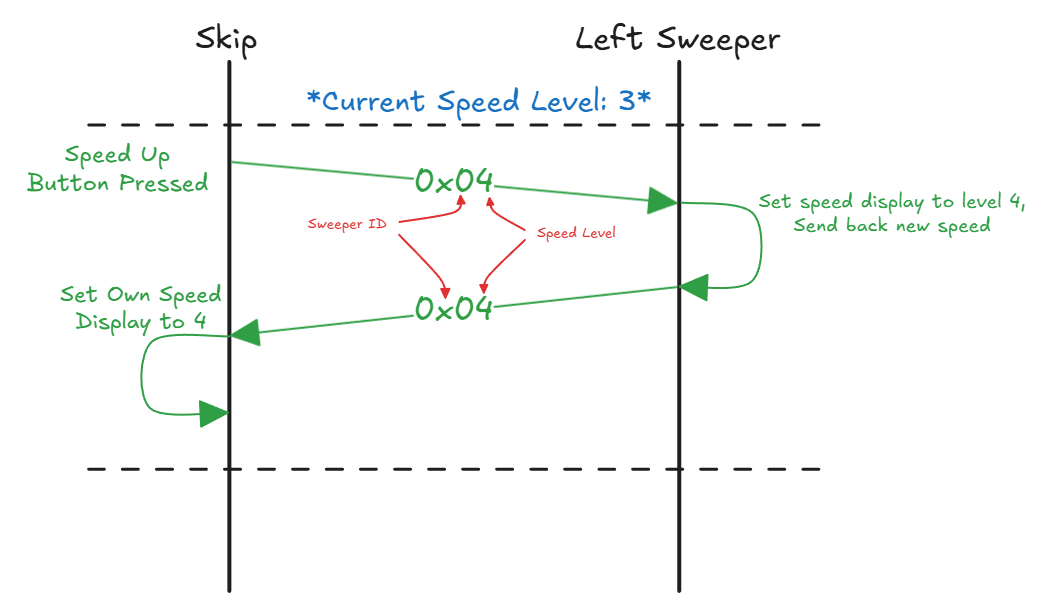
\includegraphics[width=0.6\textwidth]{message_structure_idea.png}
    \caption{Message communication diagram}
\end{figure}

Both sweepers will actively listen to all messages and only act when the \texttt{sweeper\_id} matches their own. This will ensure that the skip can communicate with both sweepers at the same time.

\logbookentry{A Compact Design}{January 28, 2025}
A more compact device for the skip could be used, where a switch can be used to toggle between the two sweepers. This would reduce the size of the device, and essentially reduces the number of components to just half. On the sweepers device a small vibration motor can be used to indicate a message has just arrived. A rough sketch is shown below for the more compact design.
\begin{figure}[ht!]
    \centering
    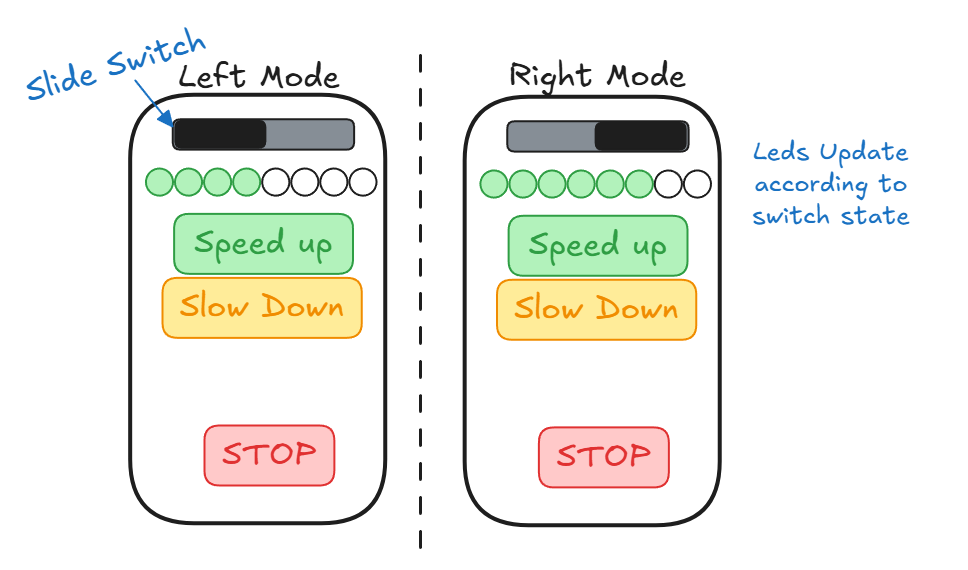
\includegraphics[width=0.8\textwidth]{design_idea2.png}
    \caption{More compact design idea}
\end{figure}

The downside I can see with this is that the skip would need to swap between the two sweepers, which could be a bit cumbersome at times. However, the size reduction could be worth it, and reduced cost of the device. It also will have less LEDs so power consumption could be reduced as well.

\section{LOGBOOK \#2 START}
\logbookentry{Design Review 1 Reflection}{February 3, 2025}
After the feedback of the initial design review, we have altered our design. Our big oversight was the huge amount of granularity we had in our design. Coming up with multiple sweeping speeds is unecessary and we have learnt that there is really only 3 levels, sweep hard, clean the ice and stop. Outside of this, the curlers will know what to do.

We also have decided to modify our design to contain simpler commands and share the same command to both sweepers. This means that if the skip wants the stone to curl left, we can send the curl left command to both sweepers, and the sweepers will know what to do to make the stone curl left. This will simplify the design and make it easier to implement.

\logbookentry{Lab 2}{February 3, 2025}
The goal of this lab was to get familiar with the ESP32 and the ESP-Now protocol.
We first decoded the positions of a joystick and then controlled LEDs on a ring based on the position of the joystick. The controller was connected to the board at 2 different ADC pins and we read the values of the x and y direction to determine the location. At each position, 8 samples were taken and averaged to get a more resistent value. The x, y values were then used to decode where the joystick was pointing and the LEDs were lit up accordingly.

To light up the LEDs I had used the adafruit neopixel library, allowing me to light any of the 12 LEDs on the ring. The position of the joystick was encoded by a value of 1-9, which represented a position on a grid that was later used to communicate with another device using ESP-Now. The encoding scheme was as follows:
\begin{table}[ht!]
    \centering
    \begin{tabular}{|c|c|c|}
        \hline
        NW & N & NE \\
        9 & 8 & 7 \\
        \hline 
        W & C & E \\
        6 & 5 & 4 \\
        \hline
        SW & S & SE \\
        3 & 2 & 1 \\
        \hline
    \end{tabular}
    \caption{Joystick encoding scheme}
\end{table}

A function was created which took a direction value, 1 through 9, and lit up the corresponding LED(s).

In the last part of the lab, we had obtained the mac address of a differnet device to communicate via ESP-Now. We established a connection between the sender and receiver and then send a message containing the encoded joystick position to the receiver. The receiver would then light up the corresponding LED on the ring. The communication was successful and the LEDs lit up as expected. There was a short delay added as to not overload the network with messages.

\textbf{Questions for Lab 2}
\begin{enumerate}
    \item The joystick was powered by the 3.3V and grounded by the GND pin. Two ADC1 pins were used to read the x and y values of the joystick. For the LED ring, the data pin was connected to a GPIO pin on the ESP32, and powered in a similar fashion to the joystick.
    \item The folow of the program is as follows:
    \begin{itemize}
        \item Connect with receiver via ESP-Now
        \item Initialize the LED ring
        \item Main Loop:
        \item Sample x and y values 8 times and average them
        \item Decode the position of the joystick into one of 9 positions
        \item Send the position to the receiver via ESP-Now
        \item Receive the position and light up the corresponding LED
    \end{itemize}

    \item To improve the usability of the device, a difference decoding scheme from the coordinates to position could be used. Currently there exists some deadzones where the joystick is close to one position but LEDs do not light up.

    \item There were no major performance issues, aside from the added delay as to not overload the network. The LEDs lit up as expected and the joystick was able to control the LEDs. Doing a serial print, it was able to detect and decode the position in a very fast manner.
    \item Technical questions:
    \begin{enumerate}[label=\alph*.]
        \item The transmitter needs to know the MAC address of the receiver because ESP-NOW does not use IP addresses like regular Wi-Fi. Instead, devices communicate directly using their unique MAC addresses. This helps the sender know exactly which device to send data to. Without the MAC address, the transmitter wouldn`'t know where to send the message. There is an option to broadcast the message to all devices by using the mac address of 0xFF.

        \item We are not able to determine if the message was received, only if it was sent succesfully. To ensure the message was received, we could implement a handshake protocol where the receiver sends an ACK message back to the transmitter. This would ensure that the message was received and understood by the receiver.
        \item \begin{enumerate}
            \item There is no way to authenticate that the packet was specifically meant for a target device if it is broadcasted. However, we can add extra details in the packet to ensure that the receiver knows that the packet was meant for them. This could be a simple ID, or a more complex encryption scheme to ensure that the packet was meant for the receiver.
            \item The transmitter would not know if the message was received by the target device by default. However, as discussed above, we can implement a handshake protocol.
            \item As more devices transmit on the network, we would have more congestion and sending messages could take longer and even fail if the network is too congested. This is why we had added an artifical delay to ensure that the network was not overloaded with messages.
        \end{enumerate}
    \end{enumerate}
\end{enumerate}

\logbookentry{Design Refinement}{February 5, 2025}
The new design idea contains a more simplified setup. 5 buttons are present on the skips device along with an LED ring. The sweepers device will be a simple case with the same LED ring. The commands will be sent to both sweepers at the same time. We will also show the command for a brief period before turning the LEDs off, which will allow for better power consumption. The different commands will light up different parts of the LEDs in various colors to make it as easy as possible for the sweepers to differentiate the different commands. The current command encoding for the LEDs is as follows. This is preliminary and could change as we test the design. The goal would be to make it as easy as possible for the sweepers to understand the command.
\begin{table}[ht!]
    \centering
    \begin{tabular}{|c|c|}
        \hline 
        \textbf{Command} & \textbf{LEDs} \\
        \hline
        Sweep Hard & Green - Fully lit \\
        Clean Ice & Blue - Top Half \\
        Stop & Red - Fully lit \\
        Curl Left & Blue - Left Half \\
        Curl Right & Blue - Right Half \\
        \hline
    \end{tabular}
    \caption{Encoding for LEDs}
\end{table}

\logbookentry{PCB Assignment}{February 9, 2025}
The PCB assignment was done succesfully without any errors. Initially I had picked the EasyEDA pro option, but then switched to the std edition as it was easier and more intuitive to use. The artistic element included on the PCB was a meme of a guy pointing towards the required information on the back of the board.

The design of the PCB is from class, a Human-Machine-Interface board with push buttons, an analog input and a screen. We utilize an OLED screen, 2 push buttons, a potentiometer and a status LED. The screen is controlled by an I$^2$C interface, the push buttons are connected to two seperate pins, and the potentiometer is connected to a different pin. A generic 8-pin header is also present to connect to a MCU to control the board.

\logbookentry{PCB Assignment - Bill of Materials}{February 11, 2025}
The bill of materials with sources for the PCB we designed as follows:
\begin{table}[ht!]
    \centering
    \begin{tabular}{|c|c|c|c|c|}
        \hline
        \textbf{Part} & \textbf{Quantity} & \textbf{Price} & \textbf{Total} & \textbf{Source} \\
        \hline
        Capacitor & 3 & \$0.03442  & \$0.10326 
        &\href{https://www.digikey.ca/en/products/detail/kemet/C0805C104K3RACTU/411167}{\underline{DigiKey}} \\
        Header Pin & 1 & \$0.11134 & \$0.11134 & \href{https://www.digikey.ca/en/products/detail/adam-tech/PH1-08-UA/9830442}{\underline{DigiKey}} \\
        Push Button & 2 & \$0.62256 & \$1.24512 & \href{https://www.digikey.ca/en/products/detail/schurter-inc/1301-9314-24/8536705}{\underline{DigiKey}}\\
        LED & 1 & \$0.18192 & \$0.18192 & \href{https://www.digikey.ca/en/products/detail/w%C3%BCrth-elektronik/150060BS55040/8557178}{\underline{DigiKey}} \\
        Resistors & 5 & \$0.00619 & \$0.03095 & \href{https://www.digikey.ca/en/products/detail/bourns-inc/CR0603-JW-102ELF/3741004}{\underline{DigiKey}} \\
        Potentiometer & 1 & \$1.40968 & \$1.40968 & \href{https://www.digikey.ca/en/products/detail/bourns-inc/3386P-1-202LF/1088527}{\underline{DigiKey}} \\
        OLED Screen & 1 & \$11.99  & \$11.99 & \href{https://www.waveshare.com/1.54inch-oled-module.htm}{\underline{Waveshare}} \\
        \hline
        \multicolumn{3}{|r|}{\textbf{Total}} & \$15.07 & - \\
        \hline
    \end{tabular}
    \caption{Bill of Materials}
\end{table}

The OLED screen was sourced from waveshare and is of the same specification as the one used in the PCB. It is a 1.54 inch OLED screen with a resolution of 128x64 pixels with an I$^2$C interface. Other parts were sourced from DigiKey, and were picked to fit the footprint on the PCB and the requirements of the board.
\newpage
\section{LOGBOOK \#3 START}
\logbookentry{Design Idea - Message Encoding}{February 17, 2025}
\autoref{fig:msg_encoding} shows how each message would be displayed on the ring. Colors and position of the LEDs are used to indicate the message. Common colors are used, as green to sweep as it normally signals go, red to stop, and orange to clean. For the curl and line commands, the right and left halves are lit up respectively. For curl we use the color blue and yellow for, which can be easily differentiated by the sweepers. 

One potential problem is that depending on the LEDs, orange and yellow may be hard to differentiate, so we may need to change the colors for the line and clean commands.
\begin{figure}[ht!]
    \centering
    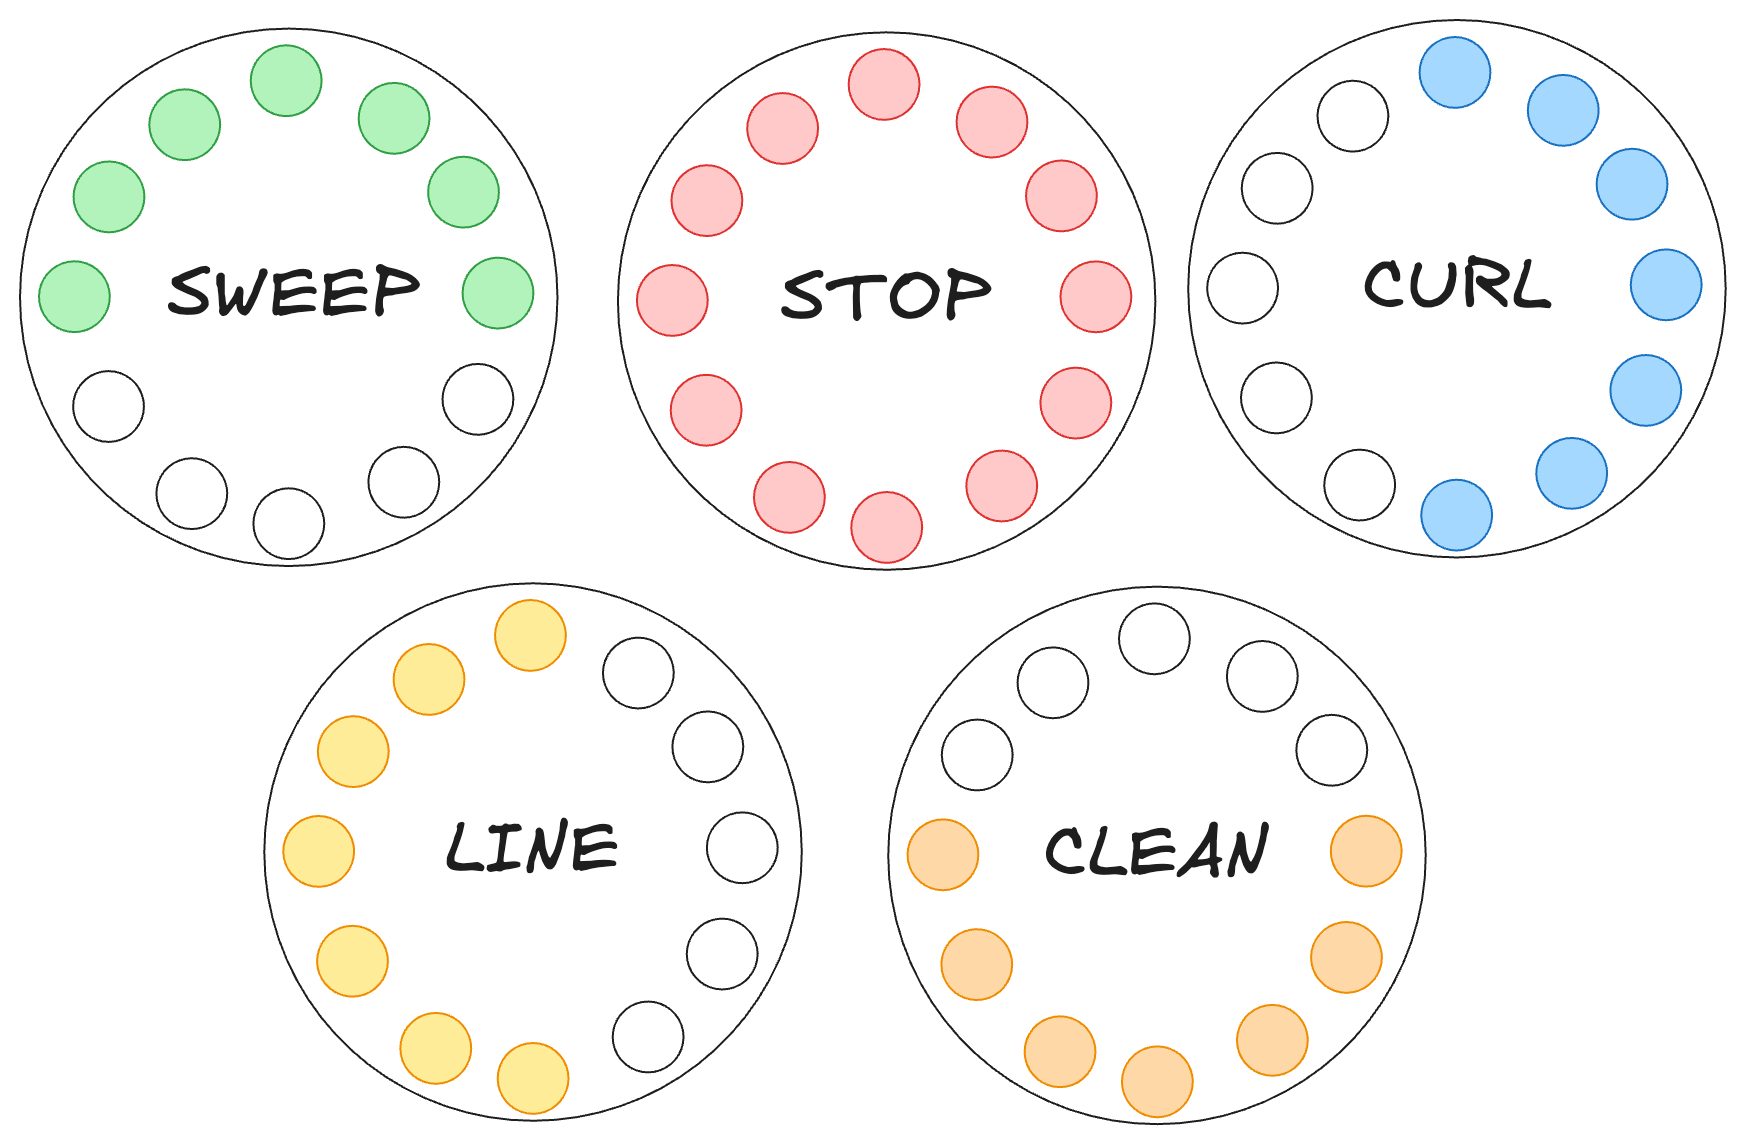
\includegraphics[width=0.35\textwidth]{msg_encoding.png}
    \caption{Message encoding on the ring}
    \label{fig:msg_encoding}
\end{figure}

\logbookentry{Design Idea - Sweeper and Skip Device}{February 20, 2025}
\autoref{fig:skip_device} shows a potential design for a more refined skip device. It is a circular device with 5 buttons on the front and an LED ring around the edge. It would have a hook at the top to allow for a lanyard or string to be attached. 

\begin{figure}[ht!]
    \centering
    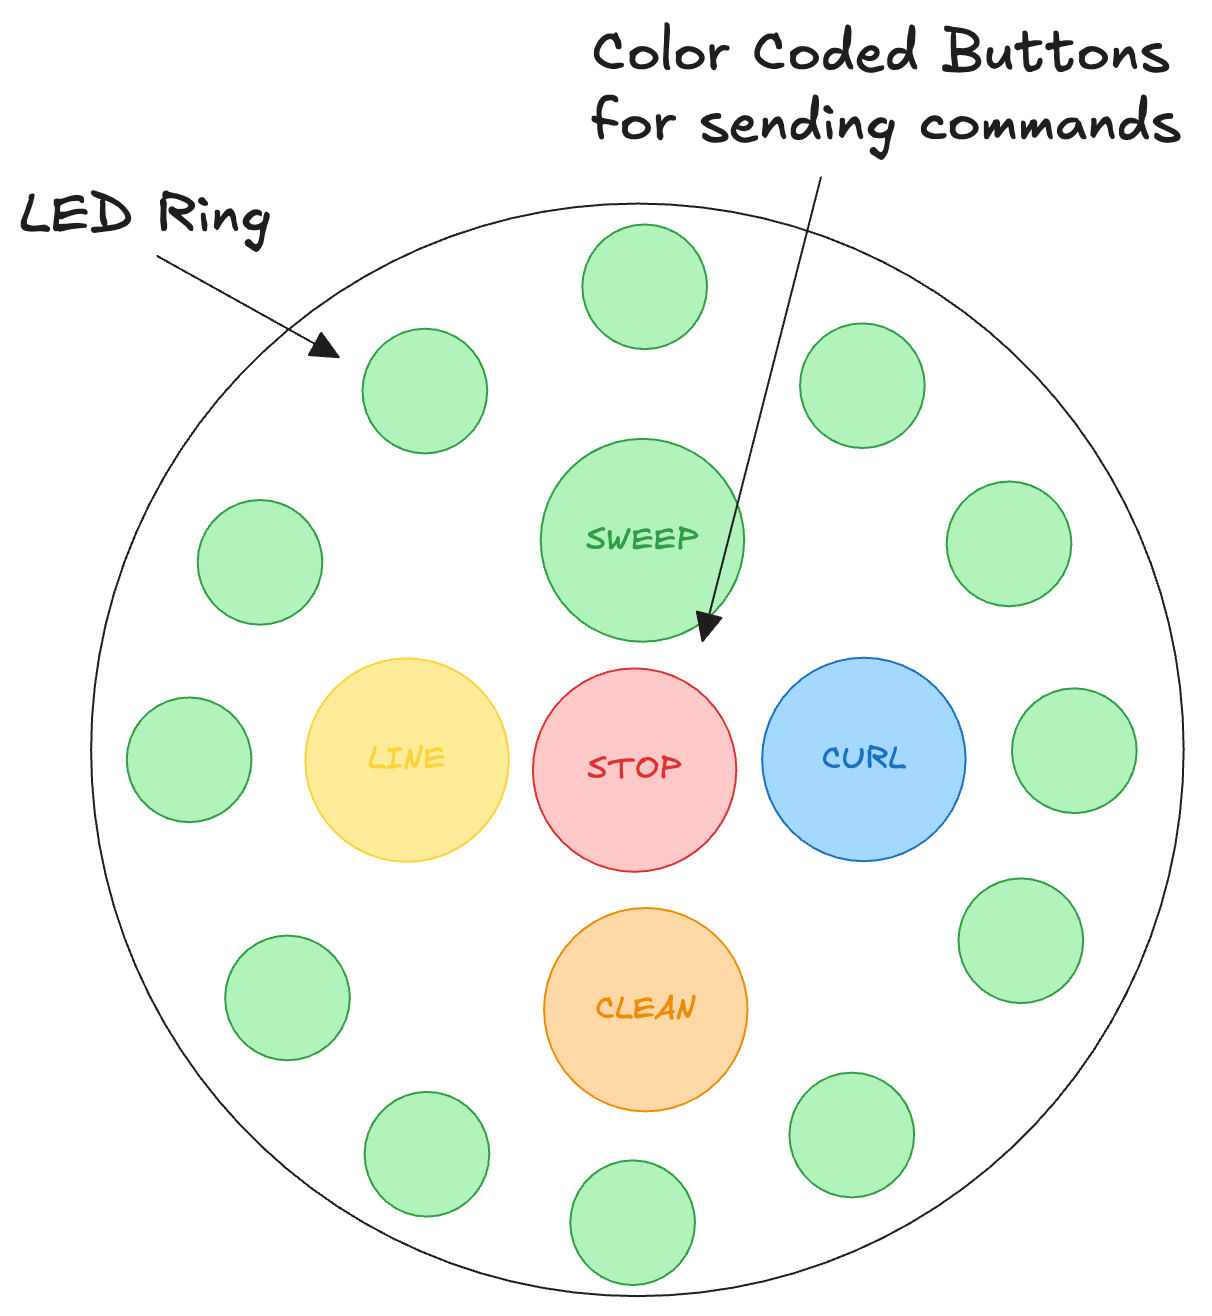
\includegraphics[width=0.35\textwidth]{skip_device.png}
    \caption{Skip device design}
    \label{fig:skip_device}
\end{figure}

For the receiver side, the sweepers device could be similar to the curling timers that get attached onto the brooms. The idea is to have the device that can be positioned at various lengths on the broom, and can be easily seen by the sweepers. The led ring wold be angled slightly towards the sweeper to make it easier to see. Similar design concept to \autoref{fig:curling_timer}, found on the internet.
\begin{figure}
    \centering
    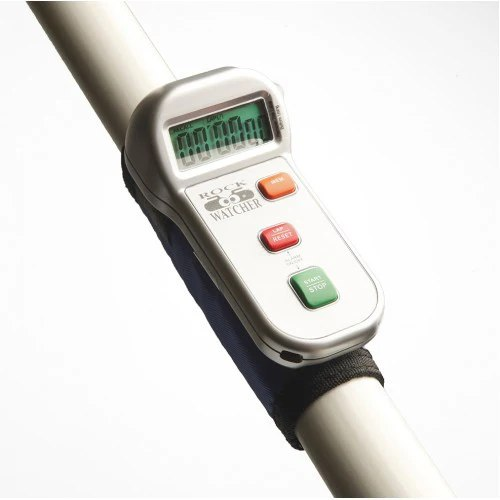
\includegraphics[width=0.35\textwidth]{curling timer.png}
    \caption{Curling timer design}
    \label{fig:curling_timer}
\end{figure}

\logbookentry{Design Idea - Sweeper device sketch}{Feb 22, 2025}

\autoref{fig:sweeper_device} shows a rough sketch of the sweeper device. As previously described, it would be a device that can be attached to the broom and would have an LED ring that would light up based on the command from the skip. 

\begin{figure}[ht!]
    \centering
    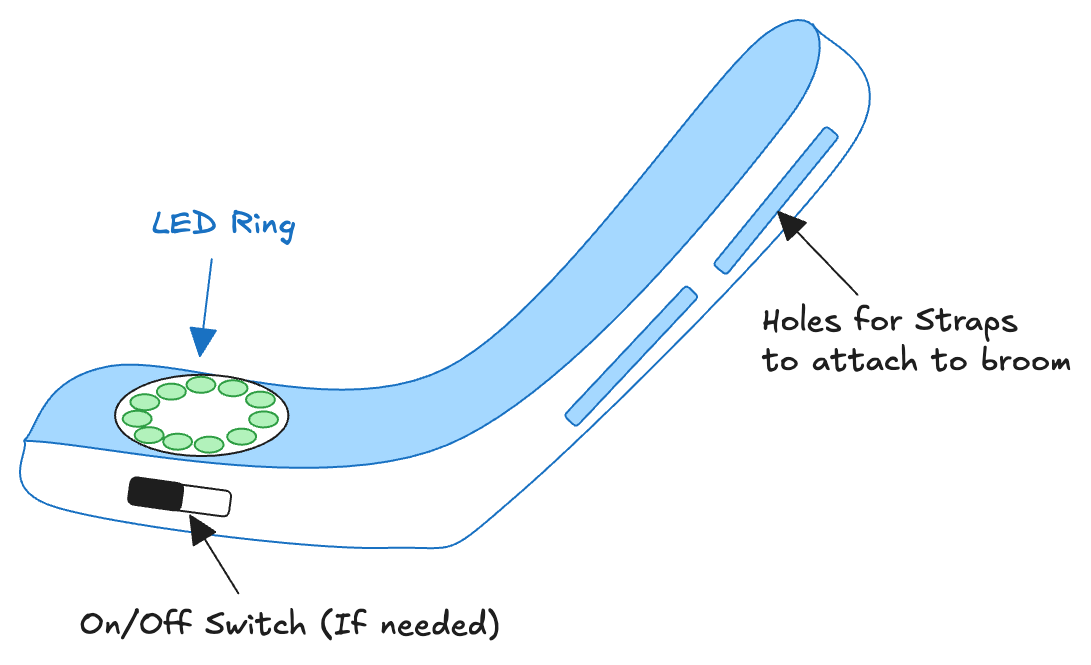
\includegraphics[width=0.35\textwidth]{sweeper_device.png}
    \caption{Sweeper device sketch}
    \label{fig:sweeper_device}
\end{figure}

Alternatively, a plastic clip could be used, instead of straps to attach the device to the broom, however this is not a very important detail at the moment. The main focus is to have a device that can be easily attached to the broom and can be easily seen by the sweepers.


\logbookentry{Lab 3}{February 24, 2025}
Lab 3 consisted of implementing power saving measures on the ESP32 with the joystick from lab 2. The goal was to see a significant improvement in the average current consumption with the power saving measures implemented. This was achieved by putting the ESP32 into a light sleep instead of a blocking delay, reducing the CPU clock frequency and WiFi power.

 
\textbf{Light Sleep}

Since the required transmition rate was every 150ms, a majority of the time was spent doing nothing, about 145ms of waiting and 5ms of processing. This was a perfect use case for light sleep, as the ESP32 could go into a this low-power idle state and wake up every 150ms to transmit the data. The delay was set to 145ms and once transmitted, the wifi was turned off and the ESP32 went into light sleep.


\textbf{Reducing CPU Clock Frequency}

Testing the power consumption at different CPU frequencies, it was found that the lowest frequency at which the radio was also operational showed the lowest power consumption. The frequency was set to 80MHz, which was the lowest frequency at which the radio was operational.

\textbf{Reducing WiFi Power}

The WiFi power was reduced to the lowest setting, which reduced the total power consumption of the ESP32.

\newpage
\textbf{Results}

The results of the power saving measures are shown in \autoref{fig:power_consumption}. The baseline power consumption was around 129.44mA, and with the power saving measures implemented, the power consumption was reduced to around 16.21mA. This was a significant improvement in power consumption and showed that the power saving measures were effective.
\begin{figure}[ht!]
    \centering
    \begin{subfigure}[b]{0.45\textwidth}
        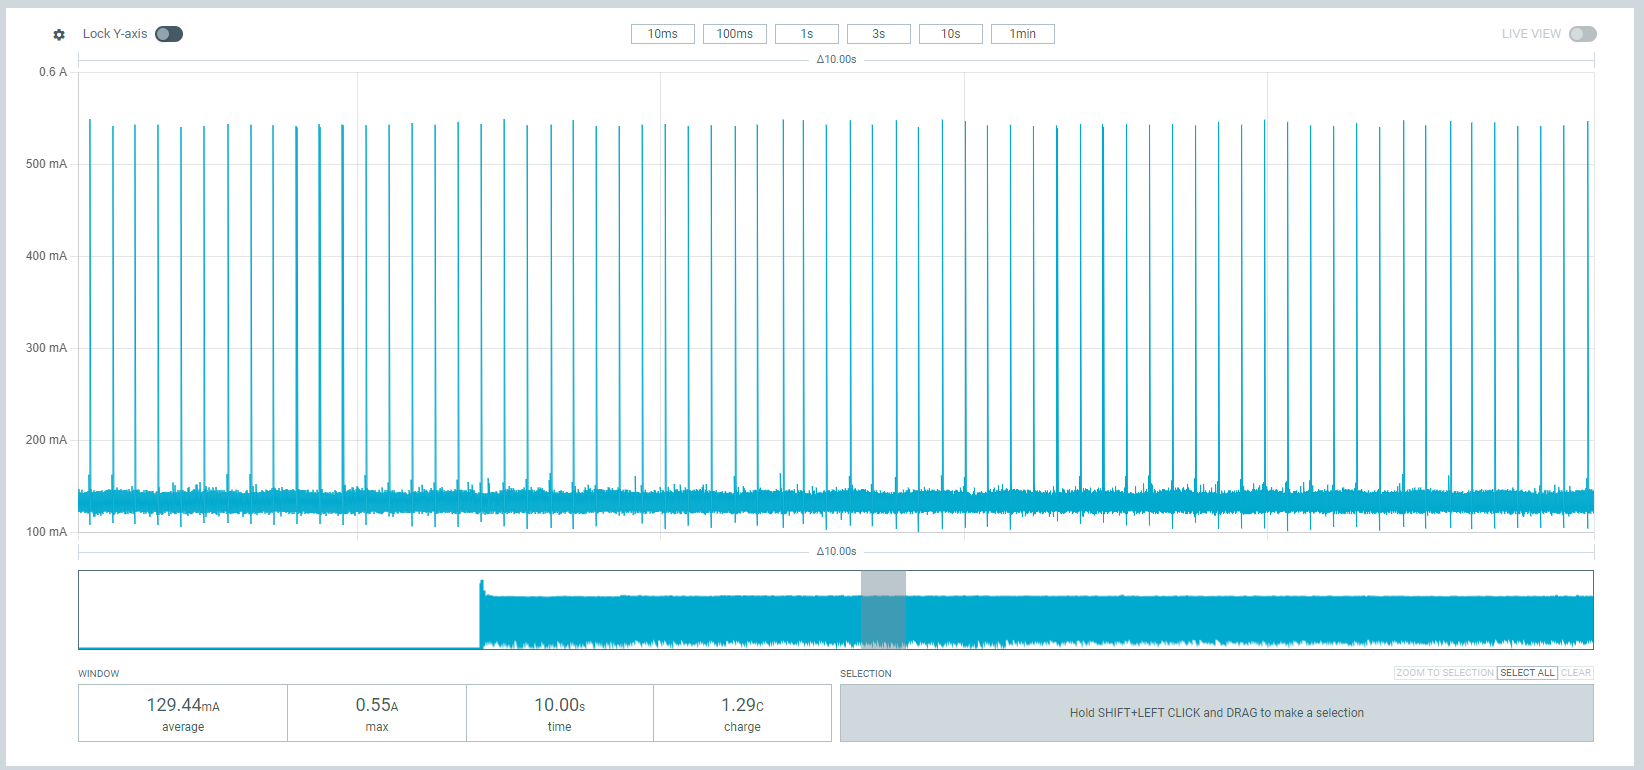
\includegraphics[width=\textwidth]{baseline.png}
        \caption{Baseline}
    \end{subfigure}
    \begin{subfigure}[b]{0.45\textwidth}
        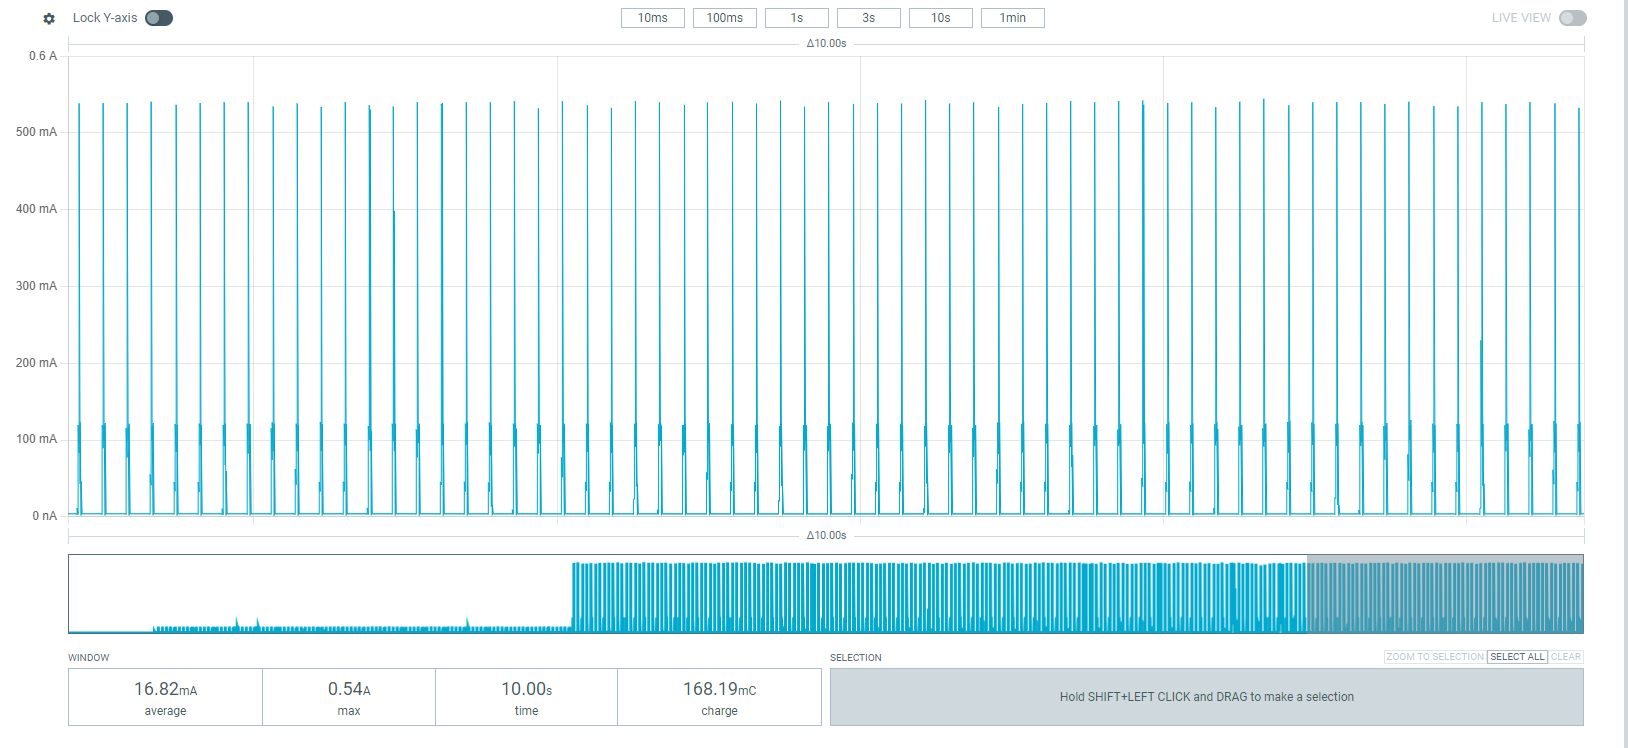
\includegraphics[width=\textwidth]{2nd benchmark.png}
        \caption{Light Sleep}
    \end{subfigure}    
    \begin{subfigure}[b]{0.45\textwidth}
        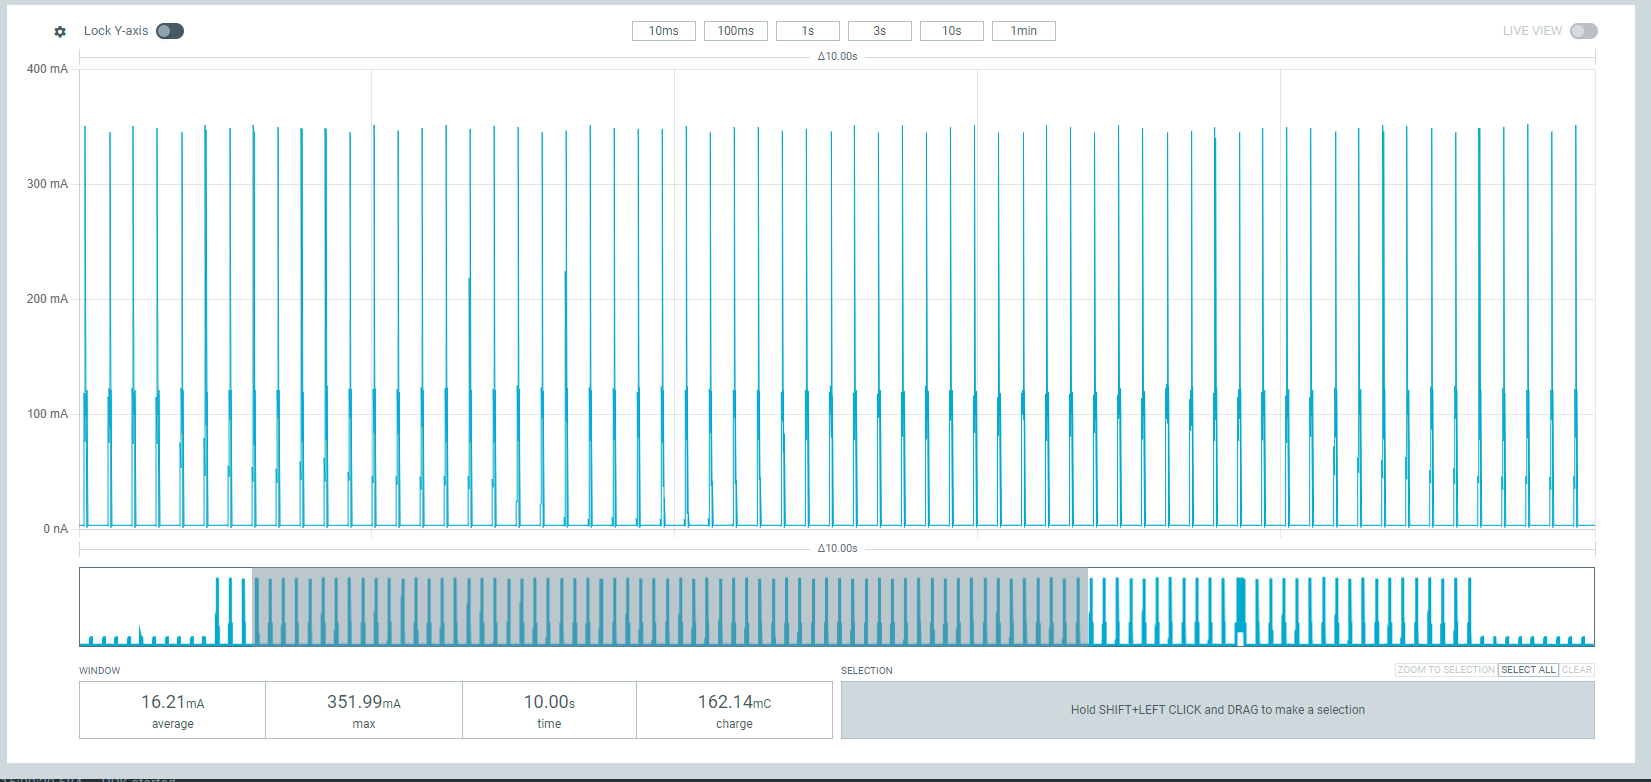
\includegraphics[width=\textwidth]{3rd benchmark.png}
        \caption{Reduced CPU Frequency + Light Sleep + Reduced WiFi Power}
    \end{subfigure}
    \caption{Current consumption}
    \label{fig:power_consumption}
\end{figure}

We will calculate the worst-case scenario for power consumption on our device. We have some push buttons which are negligible, a 12-LED ring which will consume 30mA per LED at max brightness, and 1 mA on idle. 

The sender will include the 12-led ring which gives us an idle power consumption of 12mA, and adding a little bit more for the light-sleep mode, we can assume roughly 15mA on idle. When a push button is pressed, the LEDs will light up and the message will be sent to the receiver. Assuming all LEDs are lit up, and using only 1 channel at half brightness, that is a single color (r, g or b) at 50\% brightness, we can calculate the power consumption as follows:
\begin{align*}
    \text{LED Power} &= 12\text{ LEDs} \times 10\text{ mA / LED Channel} \times{1 \text{ Channel}} \times 0.5\text{ Brightness} = 60\text{ mA} \\
\end{align*}

Since we only transmit when a button is pressed, the acive power consumption will be slightly higher than 60mA, so we can assume around 65mA, which would include the power consumption of the ESP32 and the radio to transmit the signal.

On the receiver side, we only have the 12-LED ring. Without any complex power-saving measures, the receiver will continously listen for messages and light up the LEDs. This would have the idle power consumption of 30-35mA, and when a message is received, the LEDs will light up. Assuming the same power consumption for the LEDs and slightly higher for actively listening for messages, we can assume around 75mA.

The reason for this 30-35mA idle consumption on the receiver is that we are always listening. To get past this limit, we would need to implement a synchronization method so that the receiver can sleep when it is not expecting a message. This would require something like a handshake protocol to synchronize the time and also utlize a consistent message sending rate.

If we de-age the LiPo battery to 80\% of its capacity, we can calculate the battery life as follows:
\begin{align*}
    \text{Sender Battery Life} &= \frac{500 \text{ mAh} \times 0.8}{65\text{ mA}} = 6.15\text{ hours} \\
    \text{Receiver Battery Life} &= \frac{500 \text{ mAh} \times 0.8}{75\text{ mA}} = 5.33\text{ hours}
\end{align*}

This is the worst-case scenario where the device is continously transmitting and receiving messages. In a real-world scenario, the battery life would be much longer as the device would not be continously transmitting and receiving messages. The following plot shows the battery life of the device with various active percentages.

We plot the following equation, where a = active percentage:
\begin{align*}
    \text{Sender Battery Life} = \frac{500 \text{ mAh} \times 0.8}{a \cdot 65 \text{mA} + 15 \text{mA} (1-a)} \text{ hours} \\
    \text{Receiver Battery Life} = \frac{500 \text{ mAh} \times 0.8}{a \cdot 75 \text{mA} + 35 \text{mA} (1-a)} \text{ hours} \\
\end{align*}
\begin{figure}[ht!]
    \centering
    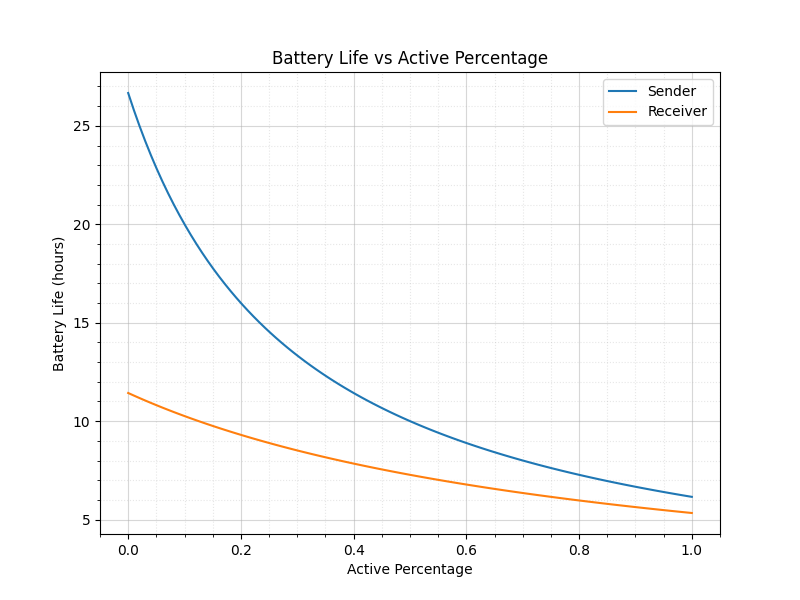
\includegraphics[width=0.5\textwidth]{battery_life.png}
    \caption{Battery life of the device}
    \label{fig:battery_life}
\end{figure}

If we assumed that it would be active 50\% of the time, we get a battery life of 10 hours on the sender and 7.27 hours on the receiver. This is a more realistic scenario where the device would not be continously transmitting and receiving messages.

\newpage
\logbookentry{3D Design Idea}{February 28, 2025}
A 3D case was made for the idea in \autoref{fig:skip_device}. It would be a small hand-held circular device with 5 buttons on the front and an LED ring around the edge. \autoref{fig:3d_design} shows the design of the device. An addition to this design is to add a hole on the side for a powerswitch, and depending on the battery type, a charging port. If a non-rechargable battery is used, then the two halves can be twisted open like a screw. A ring for a lanyard is also present at the top of the device.

\begin{figure}[ht!]
    \centering
    \begin{subfigure}[b]{0.45\textwidth}
        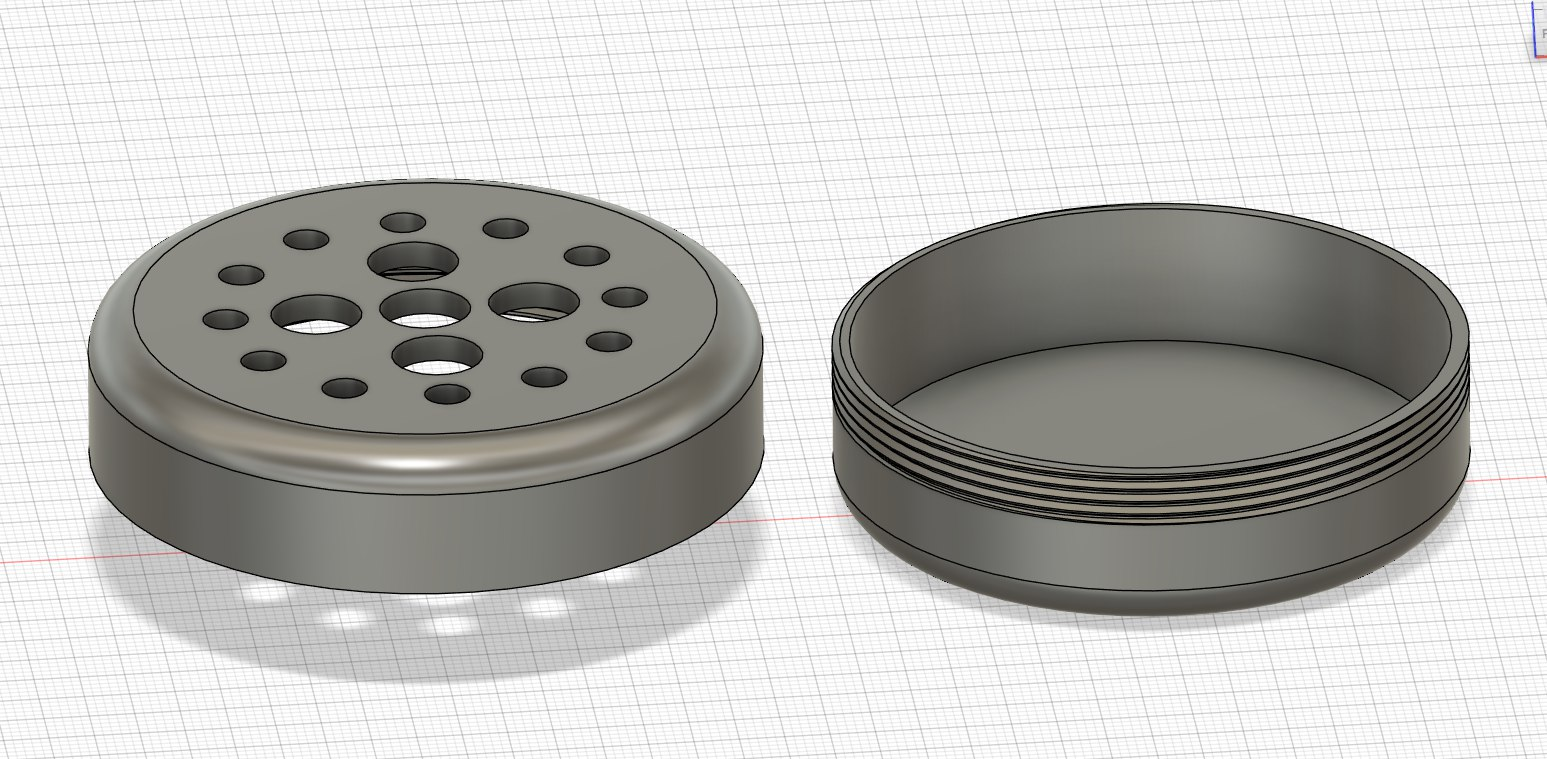
\includegraphics[width=\textwidth]{3d_design.png}
        \caption{Angled view}
    \end{subfigure}
    \begin{subfigure}[b]{0.30\textwidth}
        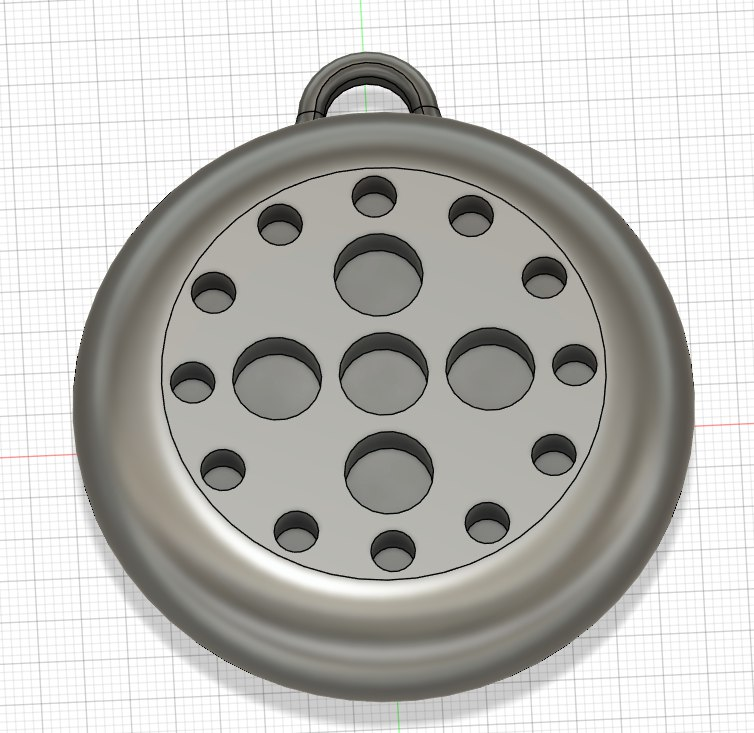
\includegraphics[width=\textwidth]{3d_design_2.png}
        \caption{Top view}
    \end{subfigure}
    \caption{3D design of the device}
    \label{fig:3d_design}
\end{figure}


\logbookentry{Lab 3 - Optimizations}{March 4, 2025}
Previously, the way the ESP-32 went to sleep was not optimized. It went to sleep after a fixed delay which caused issues when the data was not properly received. To ensure the sleep was done at the proper time, a callback was used to set off a flag when the data was succesfully transmitted. Once the flag was set, the ESP32 WiFi would be turned off and the light sleep would start with a calculated sleep time.

The sleep time is also now dynamic, where we find the amount of time processing and sending takes and subtract that from the total time we want to sleep. This ensures that the ESP32 wakes up at the proper time to send the data. That is:
\begin{align*}
    \text{Sleep Time} = 150\text{ms} - (t_{\text{end}} - t_{\text{start}})
\end{align*}
Where $t_{\text{end}}$ is the time the data was received and $t_{\text{start}}$ is when the esp initally Woke up. These times are found by utilizing the \texttt{millis()} function.

The results of this is shown in \autoref{fig:optimized_sleep}. This was also tested on a different board so the results are not directly comparable to the previous results, but were still significant. The power consumption was reduced to around 9.17 mA, which was a significant improvement over the previous results.
\begin{figure}[ht!]
    \centering
    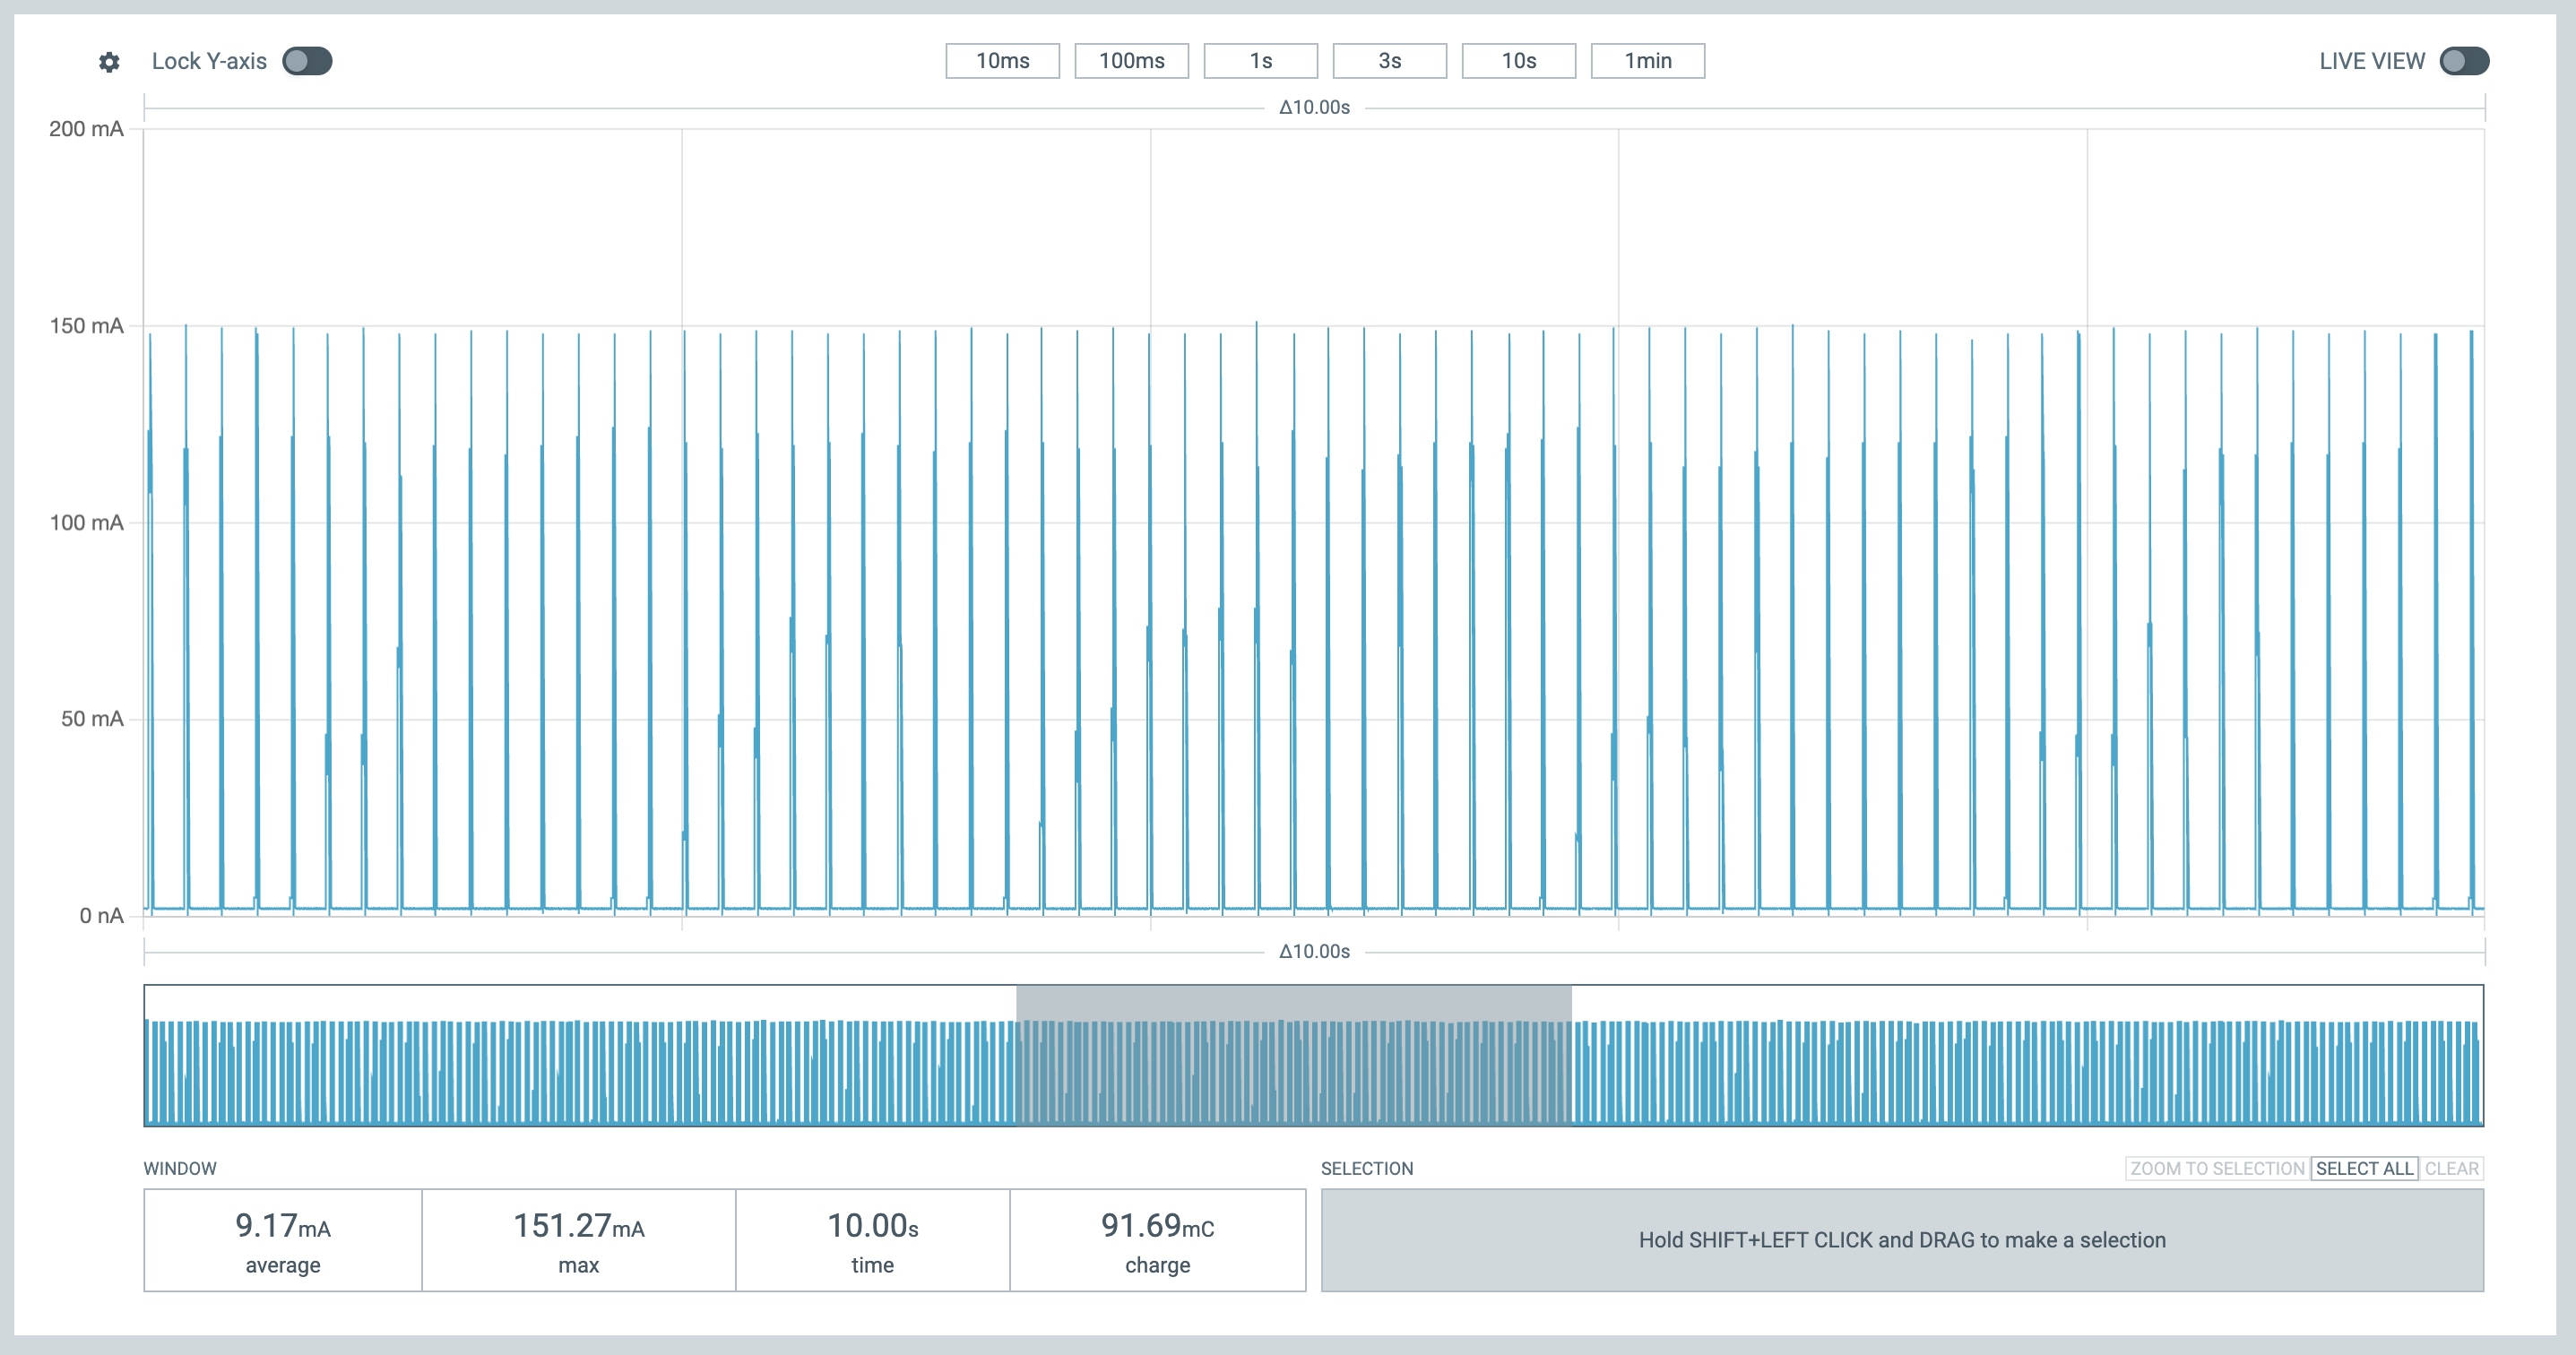
\includegraphics[width=0.70\textwidth]{4th benchmark.png}
    \caption{Current consumption with optimized sleep}
    \label{fig:optimized_sleep}
\end{figure}

\newpage
\section{LOGBOOK \#4 START}

\logbookentry{Design Review \#2 Presentation}{March 8, 2025}
Had a group meeting to help create and finalize the presentation. Discussed various power-saving measures and made changes to the design idea. We are now removing the LED ring on the skip device as the skip would not be paying much attention to the device and would be more focused on the game. With the extra space, we can space out the buttons more, which would make it easier to distinguish between the buttons

Next step is to take the feedback from the presentation and implement it into the final design.

\logbookentry{Lab 4}{March 10, 2024}
We had picked to implement problems 1B and 2. During the lab session we were able to fully finish problem 1B and get started on problem 2.

\textbf{Problem 1B}

To tackle debouncing, we kept track of a few states for each button. The same process was done for the 3 different buttons, but the response to the button press was slightly different. The following steps were used to handle the debouncing. We first check if the current button state is different from the last button state. If it is, we are now going to check if the button stays at that state for a certain amount of time. If the new states remain the same for a period of time (for us, $> 50$ms) then we can assume that the button press is valid. Then we check when the button is released, and find out if it was a short or long press. This was simply done by checking the initial time the button was pressed and the time it was released. If the time was less than 500ms, it was a short press, otherwise it was a long press.

A similar process was done for each button, but the response to the button press was different. Anytime we were in a debouncing period, we would light up led 3 despite which button was pressed.

The output was similar to the provided output, and below is the sample output for our program:
\begin{verbatim}
    Button 1 pushed @ 4821 mS, Duration: 342 mS - Short! LED1 -> Off
    Button 2 pushed @ 5224 mS, Duration: 652 mS - Long! LED2 -> Off
    Button 3 pushed @ 5876 mS, Duration: 742 mS - Long! LED1/2 -> On
    Button 1 pushed @ 6629 mS, Duration: 120 mS - Short! LED1 -> Off
    Button 1 pushed @ 7302 mS, Duration: 139 mS - Short! LED1 -> Off
    Button 1 pushed @ 7632 mS, Duration: 192 mS - Short! LED1 -> Off  
\end{verbatim}

We can utilize this debouncing method in our final project as the buttons are one of our HID devices. This will ensure that the buttons are not accidentally pressed and that the correct action is taken when the button is pressed. Another alternative is to utilize a library like the Bounce2 library, which helps make the code more readable and easier to implement.


\logbookentry{Design Review \#2 Feedback and Implementation}{March 15, 2025}
The code was finished for the skip and sweeper devices. Initially I had done a simple wake-up on button press for the skip and send the command to the sweeper. The sweeper would constantly be listening for messages and light up the LEDs based on the command. This worked as expected but the power consumption for constant listening was too high, averaging around 200mA with all LEDs on and active listening.

Even with the larger 800mAh battery, the device would not last if we were to de-age the battery by just 20\%. As mentioned during the presentation, this method would not be ideal as the device would not last the full game. The sweepers device cannot stay on for the entire time and we would need to come up with a reliable way to send commands and sleep periodically to save power.

\logbookentry{Design - Power Savings}{March 16, 2025}
To help reduce the power consumption, we need to have it so the sweeper's device is not always listening. This was achieved by sending messages at a fixed interval. When the receiver is reset and reboots, we enter a state to constantly listen. The sender will send a message to the receiver to start the sending interval. The receiver will then start a timer of 80ms and go to sleep. After 80ms, the receiver will wake up and listen for a message, perform the action and then go back to sleep. Since messages are sent every 100ms, sleeping for 80ms will minimize the chances of missing a message and will help reduce the power consumption.

On the sender's side, messages are sent every 100ms. The sender will be woken up by a button press, or a timer. If a button press is detected, the message is set to the corresponding command and is ready to be sent. Once the timer goes off, the message is sent and the sender goes back to sleep. 

This Implementation was tested to ensure that the sender was sending messages at a rate of 10 messages / second, and the receiver was receiving messages at the same rate. After several minutes of it running, the rate of messages was consistent with the expexted rate. 

As a result of this impmentation, power consumption was around 30mA on the sender and 50mA on the receiver. This was a significant improvement over the previous power consumption and would succesfully meet our requirements for the device. This should let the device last around 8 hours on a 500mAh battery, which is more than enough for a single game of curling.

The next step is to test it with 2 and 3 sweepers to ensure that the messages are sent to all 2/3 at the same interval. This should be relatively easy to implement as we have the base code for a sender and receiver, and all we would need to add is a peer-pool and add the various mac addresses to the pool.

Finally, we need to work on finishing the 3D design for the devices and hopefully get them printed. Another addition to consider is to potentially have a visual indicator to determine when the devices are all connected to the skip device, and possibly add a timeout for the LEDs to turn off after a certain period (maybe 30 seconds) of it staying on a singular command to save power.

\logbookentry{Lab 4 - Problem 2}{March 17, 2025}
\textbf{Problem 2}

This problem dealt with OTA updates for the ESP32. We had utilized the ElegantOTA library to help solve this problem. The library was easy to use and allowed for OTA updates to be done with ease. It first requires the ESP32 to be connected to Wi-Fi and then starts a webserver on which the updates can be done. Uploading a build (.bin file) to the webserver will then flash the ESP32 with the new build.

When the device is being setup, we check if a button is pressed on boot to enter the OTA mode. If the button is pressed, the device will enter the OTA mode and start the webserver. If the button is not pressed, the device will boot normally and start the program. 

We can then upload a new build with a different version and reset the device and we see in the serial output, the device is updated with the new version, and the on-board LED will blink at a different interval to indicate the new version.

We can utilize this in our final project for a few things. This can be to include different colors or patterns for the various commands. Encoding multiple button presses as a different command. If any future power saving measures are implemented, this can be used to update the devices with the new power saving measures.

A security concern with this is that the device is open to anyone on the same network to upload a new build, which can be potentially harmful. To mitigate this, we would have to look at what security measures ElegantOTA offers, or utlize a different library which is more secure.

\logbookentry{3D Design}{March 18, 2025}

Finished the 3D design of the two devices as seen in \autoref{fig:3d_render}. The skip device no longer has the LED ring and only has the 5 buttons on the front. The sweeper device remains the same. As disussed before, they would be a twist-open case, unless a different idea to open the case is thought of. The devices, taking the shape of a stopwatch, would be easy to hold and use during the game. It would also not be a distraction as stopwatches are commonly used in curling.

Furthermore, from the feedback on the design review, the attachment for the sweeper device would need to be more secure. It would be better if it is secured at the bottom of the broom instead on the broom handle itself. If we were to attach it to the broom handle, an additional supporting device would need to be made to prevent it from flopping during the game.
\begin{figure}[ht!]
    \centering
    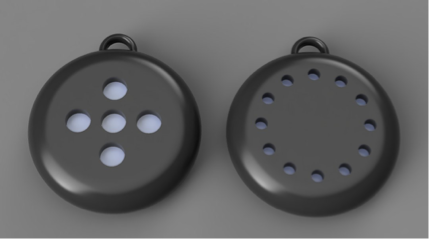
\includegraphics[width=0.45\textwidth]{design_renders.png}
    \caption{3D render of the skip (left) and sweeper (right) devices}
    \label{fig:3d_render}
\end{figure}

\section{LOGBOOK \#5 START}

\logbookentry{Printing Design and Modifications}{March 21, 2025}

The 3D design was printed but the dimensions were slightly small. The button holes were too narrow and the case was too tight for an ESP32 with all the parts to fit inside. The design was then modified by scaling everything to be 1.25x the size. The button holes were also enlarged to fit the actual dimensions of the buttons. This new design was succesfully printed and all parts properly fit. The parts are now left to be put together and assembled.

\logbookentry{Soldering and Assembly}{March 26, 2025}
The Sweeper's device was soldered and assembled. The LED ring was glued onto the case and the ESP32 was taped down to the lid of the case. The header-pins of the ESP32 were first removed and then direction connections were made to the LED ring. A foam board was also placed on the ESP32 to help keep the battery in place.

Hot glue proved to be a very useful tool in this prototyping stage. In a final design, we would implement standoffs and as screw to hold the ESP32 in place. The LED ring could also have a recessed insert to help keep it in place with  minimal gluing required.

\logbookentry{Soldering and Assembly - Part 2}{March 28, 2025}
The Skip device was also soldered and assembled but proved to be a bit more difficult. This required more wires and parts to fit in the same case as compared to the sweeper device.

All the buttons were connected in series to ground and the ESP32, and individual wires were connected from the ESP32's GPIO pins to the buttons. This was all tested to ensure every button worked and the correct command was sent to the receiver. 

One oversight of this design is the lack of access to easily turn on and off the device. A hole should've been made on the side of the devices to allow for a power switch to be added. This would make it much easier than unscrewing the device to plug/unplug the battery.

Another improvement for the design could've been to add recessed holes for the buttons to fit into. As currently they were eyeballed and glued into place, which is not the most reliable method as they are not exactly centered in the holes. Aswell, on a final design standoffs should be included to help keep the ESP32 in place, instead of taping it down. This however is a good temporary solution for our prototype and should be sufficient for our needs.

\logbookentry{Skip Code Refinement}{March 29, 2025}
As discussed in a past logbook entry, the skip device is sending commands at 10 commands / second. And this continues even when the skip is not pressing any buttons. This means if the devices are left on, the last button pressed is sent every 100ms, and the LEDs will stay on until the battery dies.

To help alleviate this, we are now keeping track of the last command that is sent and how many times in a row it is sent for. If the count of the last command is greater than 600, which is 1 minute of continously sending the same command, we switch the command to the STOP command. This will then turn of the LEDs on the sweeper device and help conserve power.

\logbookentry{Design Mold Creation}{March 30, 2025}
A mold for the skip device was designed in Fusion 360. Since the device has 2 parts, a lid and a base part, there were two seperate molds created. The lid required a two-part mold which was designed to be easily removed. The base part was designed as a three part mold due to the ring hook on one side and the threading of the screws around the device. 

More is discussed in the physical prototype assignment.

Lastly, since the device is now completed, we can test the range, battery life and other features to see if they meet our design specifications presented in the beginning of the project.


% --------------------------------------------------------------------------------
% END BODY
% --------------------------------------------------------------------------------

\end{document}


